\section{Methods}
\subsection{Walker's Alias method}

In order to generate the connections $J_{ij}$ for the dilute spin model, Walker's Alias \cite{Walker1974} method is used. This method allows us to sample random non-uniformly distributed integer numbers, i.e. rolling unfair dice in $\mathcal{O}(1)$ computation complexity with $\mathcal{O}(N^2)$ memory complexity, by splitting the sampling into rolling a fair die and then flipping a biased coin. 

\paragraph{The connection set algorithm}%
\label{sub:The connection set algorithm}

Different connections $\{i, j\}$ are drawn until $N_l$ connections have been drawn. If the connection  $\{i, j\}$ exists, discard it and try again. The algorithm to draw random connections is straight-forward: Draw an \textit{uniformly} distributed integer from 1 to N to choose the first particle. The second particle is then chosen by generating a random number $m \in [1, N-1]$, where the probability of rolling $m$ is  $P_m = m^{-(1+\sigma)}$. The sampled connection is thus $\{n, \mod(n+m, N)\}$, with $\{\}$ indicates the data structure \textit{set}. This set is stored in another set, wihch is motivated by their $\mathcal{O}(1)$ lookup time in Julia as was tested by a user \cite{setTime}. Furthermore, they are not orderered and do not have repeated elements.

The \texttt{Julia} code of the connection set algorithm is found in 

\begin{figure}[t]
	\begin{subfigure}{0.5\textwidth}
	\centering
	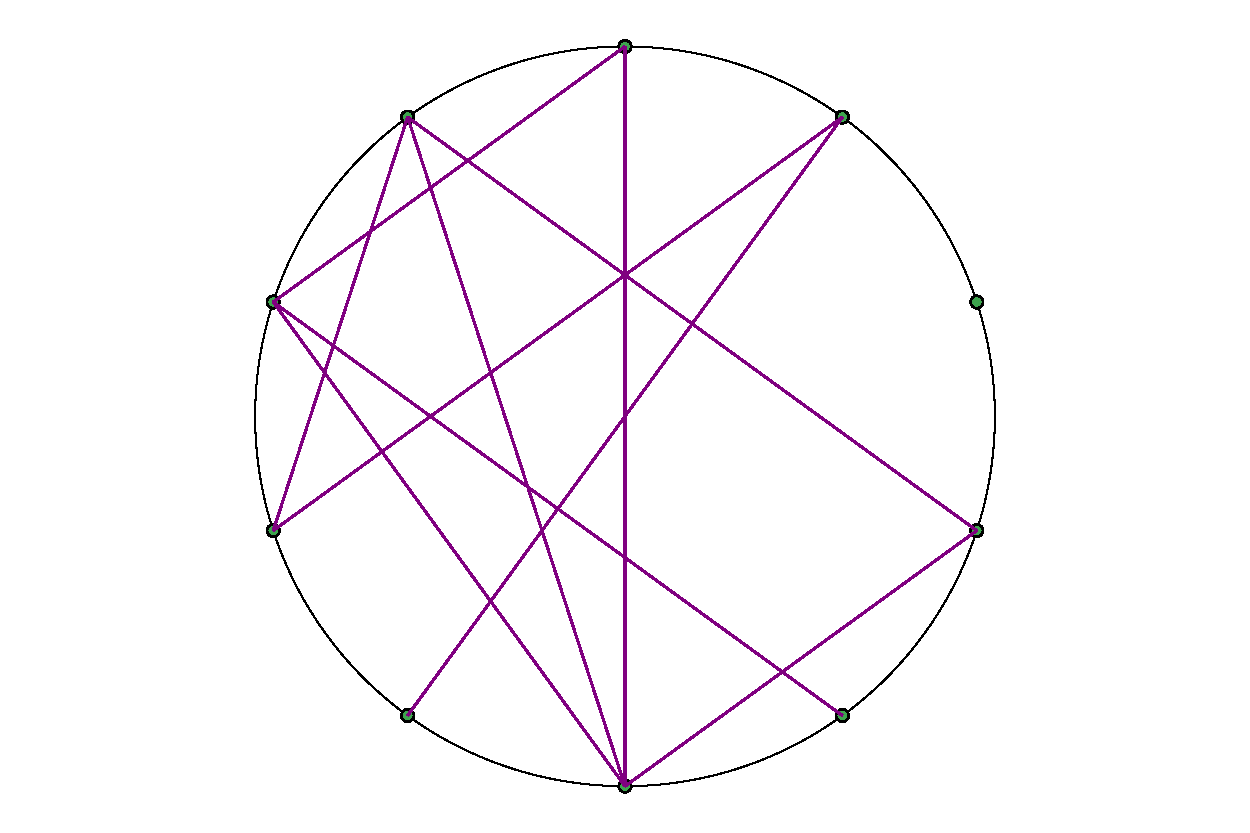
\includegraphics[width=\textwidth]{figures/partially-connected-graph.pdf}
\end{subfigure}
	\begin{subfigure}{0.5\textwidth}
	\centering
	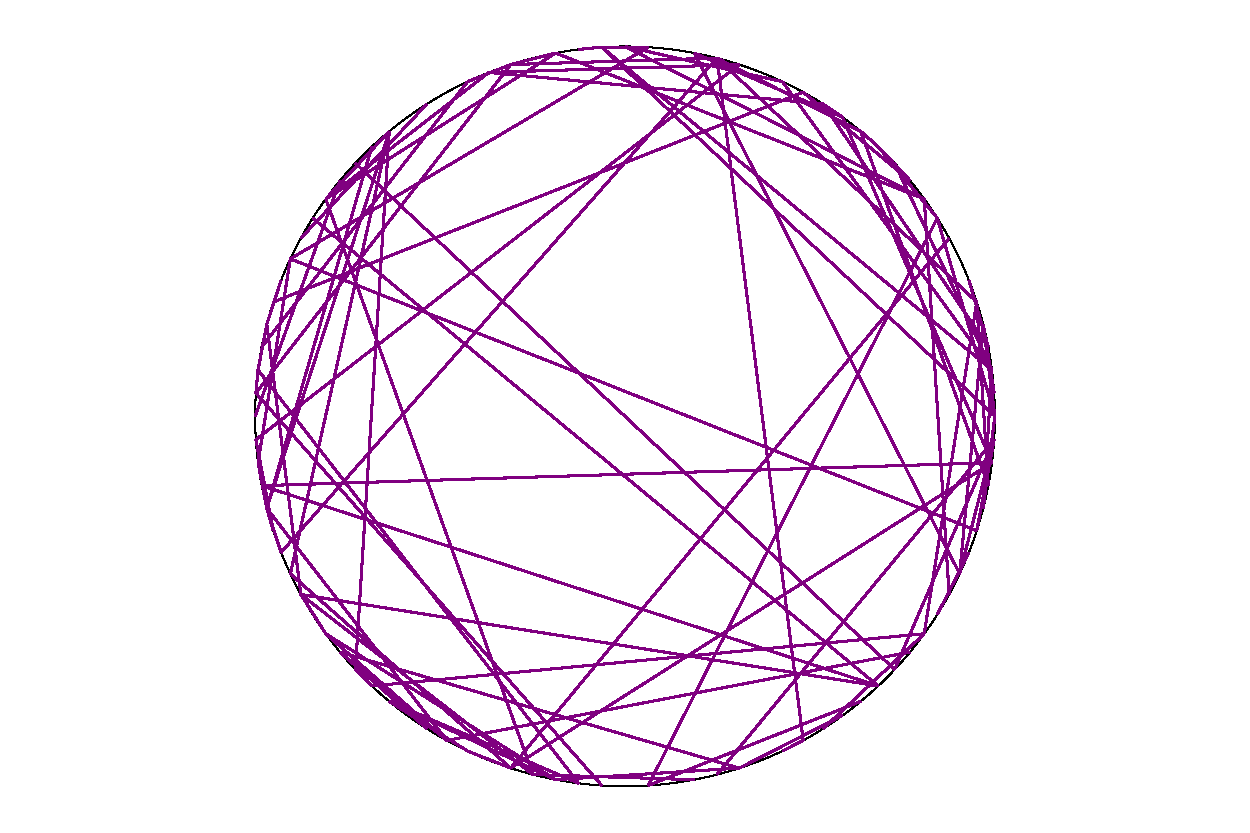
\includegraphics[width=\textwidth]{figures/partially-connected-graph-many-points-nPoints-100-nBonds-100-sigma-5.pdf}
\end{subfigure}
	\caption{Partially connected graphs of different N and $N_l$, but same $\sigma=5$. In the left panel, $N=N_l=10$, and in the right panel $N=N_l=100$.}
	\label{fig:a-partially-connected-graph}
\end{figure}

This algorithm presents the following flaw: Having to look up whether the bond (x, y) already exists in the Set is expensive (this was actually inspired from when I was using lists instead of sets, with present $\mathcal{O}(n)$ lookup time as is shown in \cite{setTime}).

This should in principle be alleviated by making the bonds in a more orderly way.
\paragraph{Pregenerated connections algorithm}

Inspired by this, I "pregenerate" the bonds. In this way, before the algorithm, the number of connections each node will have is prescribed. This connections are to be only going "forward". In an example case of nPoints = 4, nBonds = 4, this pregenerated set may look like
\begin{lstlisting}
nOfBondsList = [3, 0, 1, 0]
\end{lstlisting}
meaning the particle 1 gets three bonds, the particle 2 gets two bonds, etc.
Knowing how many bonds each particle has to get, we can do a very similar algorithm to the one before, but on a much smaller scale. The algorithm iterates over nOfBondsList, and now has to lookup in arrays of much smaller size, not $\mathcal{O}(n)$. 

\begin{lstlisting}
function walkerAliasPregeneratedConnectionsArray(nPoints,
		maxNumberOfBonds, interactionExponent)
    # My algorithm randomly chooses a point, 
    # then assigns to this point an addition index,
    # so that the addition is given by the interaction exponent.
    #
    # 1. Generate a bondsList: How many bonds 
    #       	each node is going to get connected to
    # 2. Go through each node and generate 
    # 		as many bonds as the bondsList says
    #           2.1. These bonds only go "forward"i.e. to the 
    #           	next nPoints/2 nodes
    # 3. Before each bonding, reinitialize the AliasTable,
    # 		so that the probability of 
    # 		bonding with an already bonded node is 0.

    # An nPoints long array which contains the information of how many
    # bonds each node has
    nOfBondsList = pregenerateBondsList(nPoints, maxNumberOfBonds)
    bondsList = []

    distanceAliasTable = AliasTable(
    	1 ./ distancesArray(nPoints) .^ interactionExponent
    )

    for (particle1, nBonds) in enumerate(nOfBondsList)
	if nBonds == 0
	    continue
	end
	particle1BondsList = []
	while length(particle1BondsList) < nBonds
	    particle2 = rand(distanceAliasTable, 1)[1] + particle1
	    if particle2 > nPoints
		particle2 = particle2%nPoints
	    end
	    if particle2 in particle1BondsList
		continue
	    end
	    append!(bondsList, [ sort([ particle1, particle2 ]) ])
	    append!(particle1BondsList, (particle2))
	end
    end

    bondsList
end

\end{lstlisting}



\subsection{Cluster counting}

To identify clusters we iterate over the bonds set. In this case it is way easier if we translate the connections Set (an unordered bag of (starting point, ending point) ), and we rather write the connections as an \texttt{nPoints} long array \texttt{connectivityArray}, so that  \texttt{connectionsArray[m]} is another array and its elements are the nodes to which the node \texttt{m} is connected to. In the case of a \texttt{nPoints} = 3 fully  connected graph it looks like 
\begin{lstlisting}
connectivityArray = [[2,3,4], [1,3,4], [1,2,4], [1,2,3]	
\end{lstlisting}

With the connections described in this way we perform the cluster identification using depth first search (DFS) of the set. DFS is in the worst case $\mathcal{O}(V + E)$, with V the number of vertices of the graph and E the number of edges (of each cluster). For this wee need three arrays,
\begin{enumerate}
	\item \texttt{clusters}: The identified clusters
	\item \texttt{visited}: The visitied nodes
\end{enumerate}

Starting (arbitrarily) at the first node \texttt{n=1}. Initialize a stack containig only that node. Then
\begin{enumerate}
	\item While the stack is non-empty: pop the stack (return its last element and delete it from the set). \texttt{currentElement = pop(stack)}.
	\item  If that node was not visited, add it to the current cluster, and to the \texttt{visited} set.
	\item Add the neighbours of \texttt{currentElement} to the stack. They can be retrieved from \texttt{connectivityArray[n]}.
	\item Repeat 1.
\end{enumerate}
When the stack empties it means that there are no more non-visited nodes in this cluster.

We repeat this procedure for every node, as long as that node is not in the \texttt{visited} set.

The corresponding \texttt{julia} code:
\begin{lstlisting}
function clusterIdentification(connectivityArray)
    nPoints = length(connectivityArray)
    visited = Set{Int}()
    clusters = []

    function dfs(node, cluster)
        stack = [ node ]
        while !isempty(stack)
            curr = pop!(stack)
            if !(curr in visited)
                push!(visited, curr)
                push!(cluster, curr)
                for neighbor in connectivityArray[curr]
                    if !(neighbor in visited)
                        push!(stack, neighbor)
                    end
                end
            end
        end
        cluster
    end

        for i in 1:nPoints
            if !(i in visited)
                cluster = Set{Int}()
                cluster = dfs(i, cluster)
                append!(clusters, [cluster])
            end
        end
        length(clusters)
end
	
\end{lstlisting}


